\newpage
\section{Materiais e métodos}

Uma das montagens experimentais que utilizaremos nessa prática é a do Disco de Maxwell. Ela consiste num disco que está preso a um eixo e que possui dois fios de barbante amarrados nas extremidades. Isso permite que ele seja solto de uma altura qualquer e acelere para baixo ganhando energia cinética de translação e rotação, possibilitando fazer uma análise quantitativa desses dois fenômenos. 

\begin{figure}[H]
  \centering
  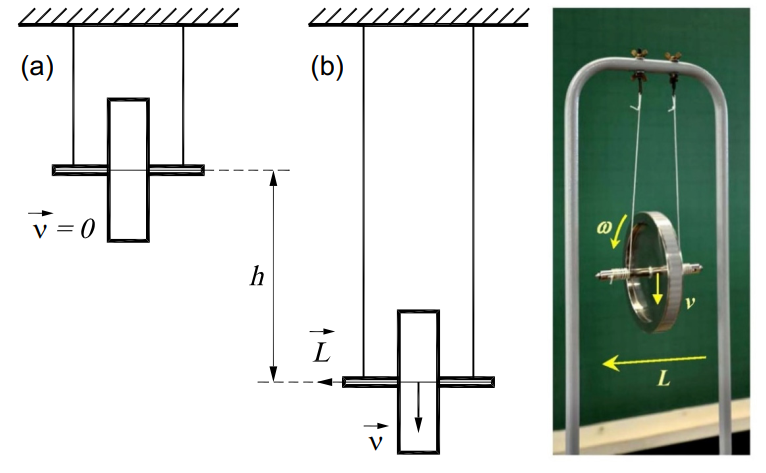
\includegraphics[scale=0.5]{images/setup-maxwell.png}
  \caption{Montagem experimental do Disco de Maxwell}
\end{figure}

% =============== EXPERIMENTO 1 ===================== %

\subsection{Determinação do Momento de Inércia de um disco}
Baseado na montagem acima, na primeira parte do experimento nós vamos calcular qual é o momento de inércia desse disco do laboratório mostrado na figura anterior.

Para isso, primeiro precisaremos determinar uma altura \textit{h} para ser o nosso referencial de energia potencial gravitacional. Podemos utilizar o fio totalmente estendido como o ponto mais baixo, e a partir daí enrolar da forma que desejar. Após escolher tal altura será feito 3 medições do tempo de queda de acordo com o esquema (a) e (b) da figura anterior. Essas medições serão feitas com um cronometro de precisão.

Com 3 valores para \textit{$t_b$} - tempo para chegar no estado (b) - encontrados, podemos calcular o valor do momento de inércia \textit{I} e a sua incerteza \textit{$\Delta$I} para cada uma das peças do disco em estudo e propagar as incertezas desse valor utilizando as seguintes fórmulas:

\[I = \left( \frac{gt_b^2}{2h} - 1 \right) mr^2\] 
\[\Delta I = \] como propaga isso??

Após os cálculos podemos enfim fazer a comparação para ver se houve ou não conservação do momento de inércia, utilizando as seguintes desigualdades:\\

formula pras desigualdades?

% =============== EXPERIMENTO 2 ===================== %

\subsection{Choques Rotacionais}
aaaaaaaaa

% =============== EXPERIMENTO 3 ===================== %

\subsection{Conservação do Momento Angular}
aaaaaaaaaa

% =============== EXPERIMENTO 4 ===================== %

\subsection{Precessão do Giroscópio}
aaaaaaaaa
